\documentclass[fullpage]{article}
	\addtolength{\oddsidemargin}{-.875in}
	\addtolength{\evensidemargin}{-.875in}
	\addtolength{\textwidth}{1.75in}

	\addtolength{\topmargin}{-.875in}
	\addtolength{\textheight}{1.75in}

\makeatletter
\setlength{\@fptop}{0pt}
\makeatother
\usepackage[utf8]{inputenc}
\usepackage[pdftex]{graphicx}
\usepackage{mathtools}
\usepackage{float}
\usepackage{amsfonts}
\usepackage{subcaption}


\title{\textbf{Computational Robotics} \\ \large Lab 1 - Markov Decision Processes}
\author{Andrew Choi}
\date{October 2019}

\begin{document}
\maketitle

\section{Introduction}

This goal of this lab is to explore finite Markov Decision Processes to control a simple discretized robot. To do so, a gridworld is constructed with well-defined boundaries and rewards. In this gridworld, we develop and implement a model for robot behavior and use it to accomplish a prescribed task.

\section{Mathematical Formulation}

\subsection{Markov Decision Processes}
Before delving into the details of the experiment, the finite Markov Decision Process as well as the methods employed (value iteration and policy iteration) are described mathematically.

Markov decision processes (abbreviated MDP from hereon) are a classical formalization of sequential decision making. Driven by rewards, these decisions are made not just influenced by immediate rewards, but also by possible future rewards. The MDP can be described as a tuple
\[
(S, A, P, R, H, \gamma),
\]
where $S$ is the state space, $A$ is the action space, $P$ is the transition probabilities between states given a certain action, $R$ is the immediate reward received from transitioning to a certain state, $H$ is the horizon, and $\gamma$ is the discount factor. With the following parameters, the goal of an MDP is to find an optimal policy $\pi^*(s)$ that outputs the best action for every state in the state space. To find such a policy, we introduce the concept of value functions in the next section and explain its role in deriving the optimal policy.  

\subsection{Value Functions and Policies}
This formulation allows us to construct a value function $V(s) \; \forall s \in S$, which is the expected discounted returns for every state.
\[
V^\pi = \mathbb{E}[\sum_t \gamma^t r(s_t)]
\]
This value function is different depending on the policy $\pi(s)$ which deterministically chooses an action depending on the current state. Using the value function, we can compute optimal policies for finite state spaces using two methods, policy iteration and value iteration. It should be noted that for these two methods to converge to an optimal policy, the state space must be discrete and computationally finite and a perfect model of the world must be provided.

\begin{figure}[H]
\centering
\includegraphics[width=60mm]{images/agent_env_relation.jpg}
\caption{The agent-environment interaction in a Markov decision process.}
\label{fig:gridworld}
\end{figure}

\subsection{Policy Iteration}
For policy iteration, an initial policy is randomly intialized. Afterwards, a two step loop starts until an optimal policy is reached. This loop consists of

\begin{enumerate}
\item Policy Evaluation $\rightarrow$ Computing $V^\pi$ for the current policy
\item Policy Improvement $\rightarrow$ Using knowledge gained from the policy's value function to improve the policy
\end{enumerate}

Policy evaluation consists of its own iterative loop in which the value function for the policy is computed using the Bellman operator in which each loop step can be thought of as extending the time horizon starting from 0 towards $H$. With each step, we use the previous value function estimate to obtain a new value function which propagates the rewards throughout the states encountered.
\[
V^\pi = \mathbb{E}_{s'}[r(s, a, s') + \gamma V(s')]
\]

Once a value function for a policy is computed, policy improvement can then be undergone to create a new improved policy. This is done by analyzing the value function and changing actions for certain state if they lead to a higher expected discounted return.
\[
\pi^{i+1} = argmax_a V^{\pi_i}(s)
\]

This iterative loop ends when the policy no longer changes. This can be thought of as being due to convergence to the optimal value function.
\begin{gather}
\lVert V^{H+1} - V^H \lVert < threshold \\
V^* = V^{H+1} \\
\pi^* = \pi^{H+1}
\end{gather}

\subsection{Value Iteration}

In contrast with policy iteration, value iteration never explicity deals with a policy. Instead the Bellman operator is applied to an initialized value function iteratively until the value function converges to the optimal value function. From this optimal value function, an optimal policy can be generated.

\begin{gather}
V_0^*(s) = 0 \; \forall s \in S \\
V_1^*(s) = {max}_a \mathbb{E}_{s'}[r(s, a, s') = {max}_a \sum_{s'} P_{sa}(s') r(s, a, s') \\
V_{H+1}^*(s) = {max}_a \sum_{s'} P_{sa}(s') [r(s, a, s') + \gamma V_H^*(s')] \\
stop \; when \;  \lVert V^{H+1} - V^H \lVert < threshold \\
\pi^*(s) = argmax_a V^*(s)
\end{gather}


\section{Experimental Setup}

\subsection{Robot Description}

For the experiment, a simple robot is is considered that will reside in the gridworld and attempt to reach a prescribed goal state. The robot will occupy one grid in the gridworld at any given time and can face any of the twelve headings identified by the hours on a clock $h \in \{0...11\}$. Each action is characterized by a movement value of 1, -1, or 0 which can be thought of as moving forward, backward, or staying still, respectively. This movement is then followed by a rotation of 1, -1, 0 which can be thought of as clockwise, counter-clockwise, and no rotation. Following this, it can be seen that the action of the robot can be described as a tuple
\[
(a, b),
\]
where $a$ is the movement value and $b$ is the rotation value. The following restrictions are applied to the robot's actions:
\begin{enumerate}
\item Attempting to move off the grid results in no linear movement, but the rotation portion will still happen.
\item Aside from restriction 1, the robot can only rotate if it also moves forwards or backwards.
\item If the robot chooses to move, a pre-rotation error may occur with probability $p_e$
\begin{enumerate}
\item With probability $p_e$ each, robot will first rotate by +1 or -1 before it moves. No pre-rotate with probability $1-2*p_e$.
\item Choosing to stay still will not incur an error rotation.
\end{enumerate}
\end{enumerate}

Then, it can be seen that the robot is defined by the following discrete action space.
\[
(1, 0), (1, 1), (1,-1), (0,0), (-1,0), (-1,1), (-1,1) \; N_e = 7
\]

The discrete state space is the set of all possible (x, y) positions and heading angles. Following this, the state space size can be computed as
\[
N_s = X*Y*R = 8*8*12 = 768
\]

\subsection{Created Gridworld and Rewards}
To allow for trajectory simulation, an 8x8 gridworld is constructed. Provided for us are the defined rewards for the states of the gridworld as shown in figure 2.

\begin{figure}[t!]
\centering
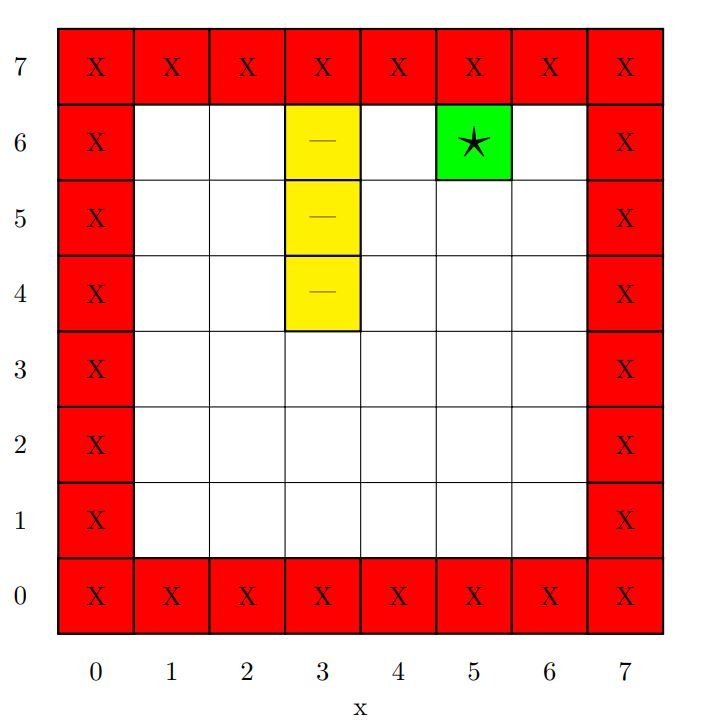
\includegraphics[width=60mm]{images/gridworld.jpg}
\caption{Gridworld with set Rewards}
\label{fig:gridworld}
\end{figure}

As the rewards for each state are independent of heading angle, they can be represented graphically on a 2D grid image. As shown above, the boundary states (red and marked X) have a reward of -100. The lane markers (yellow and marked -) have reward -10. Finally, the goal square (green and marked *) has reward +1. All other states have reward 0.

\subsection{Benchmark}
To be able to properly analyze the benefits provided by following an optimal policy, we first must set a benchmark. This benchmark will be the trajectory generated by a hand-engineered initial policy $\pi_0$. This policy crudely gets to the goal state by simply prioritizing closing the x distance and then the y distance without any regard for rewards \textit{(code in utils.py)}. The plotted trajectory can be seen in figure 2.

\subsection{Scenarios}
With the following setup, we will explore four different scenarios:
\begin{enumerate}
\item Reward at goal state located at (x=1, y=1) independent of heading, $p_e = 0\%$
\item Reward at goal state located at (x=1, y=1) independent of heading, $p_e=25\%$
\item Reward at goal state +1 only when robot is pointing down $h=6$, $p_e=0\%$
\item Reward at goal state +1 only when robot is pointing down $h=6$, $p_e=25\%$
\end{enumerate}

In addition to this, all four scenarios will start out at an initial state of $(x=1, y=6, h=6)$. A discount factor of $\gamma = 0.9$ is also employed for all scenarios. Code has been generated that can graphically plot and generate trajectories according to the different parameters above. In the next section, we analyze the results of such trajectories and discuss the significance that arises from such results. We also discuss any notable computational differences between the two methods using Python's time library.

\section{Experimental Results}

\subsection{Scenario 1}

\begin{figure}[H]
\begin{subfigure}{.5\textwidth}
\centering
\includegraphics[width=75mm]{images/pe0_ip.jpeg}
\caption{Initial Policy Trajectory}
\label{fig:a}
\end{subfigure}
\begin{subfigure}{.5\textwidth}
\centering
\includegraphics[width=75mm]{images/pe0_pi.jpeg}
\caption{Policy Iteration Trajectory}
\label{fig:b}
\end{subfigure}
\begin{subfigure}{.5\textwidth}
\centering
\includegraphics[width=75mm]{images/pe0_vi.jpeg}
\caption{Value Iteration Trajectory}
\label{fig:c}
\end{subfigure}
\caption{Scenario 1 Trajectory Results}
\end{figure}

Generated trajectories can be seen above in figure 3 for when $p_e = 0\%$ and the goal state is independent of robot heading. With $p_e$ equaling zero, this effectively eliminates any stochasticy in our environment and thus, the above trajectories will be identical if generated again since our actions deterministically get us to the state we desire. In subfigure a, it can be seen that the initial policy does fairly well, but takes an unnecessarily wide turn around the lane markers resulting in a total of +1 reward over 14 time steps to reach the goal. In contrast, both value iteration and policy iteration, result in a total of +1 reward while taking only 10 time steps to reach the goal by optimizing to take the tightest possible turn around the lane markers. In fact, the trajectories for both methods are actually identical. Although they are identical, it should be noted that each method may come up with different optimal policies as often there are multiple optimal policies for a single optimal value function as discussed earlier in section 2.2.2.
To compare computational differences, the runtimes for both methods to convergence were measured over ten separate runs and averaged with the results being as follow.
\[
PI_{time} = 6.201 \; seconds \; \; VI_{time} = 6.323 \; seconds
\]
With a difference of only about a tenths of a second, there seems to be no noticeable difference in terms of computational speed between the two methods for scenario 1. As the state space is at a manageable size, we are most likely not to see noticeable differences until the state space rises in magnitude.

\subsection{Scenario 2}

For scenario 2, we not introduce stochasticity to the environment by setting the $p_e$ to 25\%. Due to this stochasticy, different runs will result in different trajectories. Therefore, we include two plots each for the benchmark initial policy, policy iteration, and value iteration as shown in figure 4 to have a more comprehensive representation of possible trajectories. The results of the six shown trajectories can be summarized as follow.
\begin{table}[H]
\centering
\begin{tabular}{lll}
\hline
Trajectory & Total Reward & Number of Time Steps to Goal \\ \hline
IP Traj 1 & -19          & 18                           \\
IP Traj 2 & -9           & 6                            \\
PI Traj 1 & +1           & 32                           \\
PI Traj 2 & +1           & 14                           \\
VI Traj 1 & +1           & 18                           \\
VI Traj 2 & +1           & 18                          
\end{tabular}
\caption{Scenario 2 Trajectory Results}
\end{table}

At first glance, one thing that all the trajectories have in common is the fact that they often have detours and must turn around or even end up in cyclical paths due to random chance rotations. Unique to the initial policy, is that it often runs into lane markers accruing negative reward during its episode. In contrast, both value iteration and policy iteration successfully avoid negative reward states even if it ends up increasing the time it takes to the goal, since we have not assigned a penalty for increasing number of time steps for this environment. Differences in trajectory between policy iteration and value iteration are arbitrary and are due to complete chance. The important takeaway is that regardless of which method is used, both will produce policies that maximizes the reward. Compared to scenario 1, we now start to see a noticeable difference in computational time as shown below.
\[
PI_{time} = 10.492 \; seconds \; \; VI_{time} = 6.664 \; seconds
\]
laksdfkljsdflkjsdjkf

\begin{figure}[H]
\begin{subfigure}{.5\textwidth}
\centering
\includegraphics[width=75mm]{images/pe25_ip.jpeg}
\caption{Initial Policy Trajectory 1}
\label{fig:1a}
\end{subfigure}
\begin{subfigure}{.5\textwidth}
\centering
\includegraphics[width=75mm]{images/pe25_ip2.jpeg}
\caption{Initial Policy Trajectory 2}
\label{fig:1b}
\end{subfigure}
\begin{subfigure}{.5\textwidth}
\centering
\includegraphics[width=75mm]{images/pe25_pi.jpeg}
\caption{Policy Iteration Trajectory 1}
\label{fig:2a}
\end{subfigure}
\begin{subfigure}{.5\textwidth}
\centering
\includegraphics[width=75mm]{images/pe25_pi2.jpeg}
\caption{Policy Iteration Trajectory 2}
\label{fig:2b}
\end{subfigure}
\begin{subfigure}{.5\textwidth}
\centering
\includegraphics[width=75mm]{images/pe25_vi.jpeg}
\caption{Value Iteration Trajectory 1}
\label{fig:3a}
\end{subfigure}
\begin{subfigure}{.5\textwidth}
\centering
\includegraphics[width=75mm]{images/pe25_vi2.jpeg}
\caption{Value Iteration Trajectory 2}
\label{fig:3b}
\end{subfigure}
\caption{Scenario 2 Trajectory Results}
\end{figure}


\subsection{Scenario 3}

For scenario 3, we return to a deterministic setting by setting $p_e$ back to 0. For this scenario, rather than comparing to the initial policy's trajectory as the benchmark, we compare the trajectories produced by value and policy iteration to those produced in scenario 1. The trajectories are shown in figure 5. Comparing the two scenarios, the trajectories are exactly identical aside from the robot's heading. It can be seen that in scenario 1, since the goal state was independent of the robot's heading angle, the robot arbitrarily moved "forwards" while facing up. In contrast, due to the goal state requiring the robot to be in the $h=6$ heading position, the robot takes advantage of its ability to move backwards to align itself in correct orientation without sacrificing time efficiency. Much like before, we store the computational times as the average of 10 runs.

\[
PI_{time} = 10.048 \; seconds \; \; VI_{time} = 7.016 \; seconds
\]

\begin{figure}[H]
\begin{subfigure}{.5\textwidth}
\centering
\includegraphics[width=75mm]{images/pe0_pi_s3.jpeg}
\caption{Policy Iteration Trajectory}
\label{fig:a}
\end{subfigure}
\begin{subfigure}{.5\textwidth}
\centering
\includegraphics[width=75mm]{images/pe0_vi_s3.jpg}
\caption{Value Iteration Trajectory}
\label{fig:b}
\end{subfigure}
\caption{Scenario 3 Trajectory Results}
\end{figure}

\subsection{Scenario 4}

Finally, we analyze the results of scenario 4. Much like scenario 2, we show two trajectories each for value and policy iteration to get a better representation of trajectory possibilities. Furthermore, we will compare the results of both methods to those in scenario 2. Quite easily the most difficult scenario for the robot to solve, the results of scenario 4 show 


\begin{table}[H]
\centering
\begin{tabular}{lll}
\hline
Trajectory & Total Reward & Number of Time Steps to Goal \\ \hline
PI Traj 1  & +1           & 42                           \\
PI Traj 2  & +1           & 12                           \\
VI Traj 1  & +1           & 26                           \\
VI Traj 2  & +1           & 14                          
\end{tabular}
\caption{Scenario 4 Trajectory Results}
\end{table}

\begin{figure}[H]
\begin{subfigure}{.5\textwidth}
\centering
\includegraphics[width=75mm]{images/pe25_pi_s4.jpeg}
\caption{Policy Iteration Trajectory 1}
\label{fig:2a}
\end{subfigure}
\begin{subfigure}{.5\textwidth}
\centering
\includegraphics[width=75mm]{images/pe25_pi2_s4.png}
\caption{Policy Iteration Trajectory 2}
\label{fig:2b}
\end{subfigure}
\begin{subfigure}{.5\textwidth}
\centering
\includegraphics[width=75mm]{images/pe25_vi_s4.jpeg}
\caption{Value Iteration Trajectory 1}
\label{fig:3a}
\end{subfigure}
\begin{subfigure}{.5\textwidth}
\centering
\includegraphics[width=75mm]{images/pe25_vi2_s4.png}
\caption{Value Iteration Trajectory 2}
\label{fig:3b}
\end{subfigure}
\caption{Scenario 4 Trajectory Results}
\end{figure}

\section{Conclusion}

\section{Sources}

Sutton, R. S. and A. G. Barto. 2017. Reinforcement Learning: An Introduction (2nd Edition, in progress). MIT Press.


\end{document}